%------------------------ Packages ------------------------
\documentclass[12pt,a4paper]{article}
\usepackage[latin1]{inputenc}
\usepackage[T1]{fontenc}
\usepackage[pdftex]{graphicx}
\usepackage{float}
\usepackage{amsmath}
\usepackage{amssymb}
\usepackage[FIGTOPCAP]{subfigure}
\usepackage{color}
\usepackage[hidelinks]{hyperref}

\newcommand{\version}{\IfFileExists{../../version.txt}
{\input{../../version.txt}}
{\input{../../../version.txt}}
}

\newcommand{\command}[1]{%
\indent \fcolorbox{black}{white}{%
   \begin{minipage}{\dimexpr\textwidth-\parindent\relax}%
      #1
   \end{minipage}%
}
}

\newsavebox{\FVerbBox}
\newenvironment{sample}
{\par \vspace{0.2cm} \begin{lrbox}{\FVerbBox}
\begin{minipage}{\dimexpr\textwidth-\parindent\relax}}
{\end{minipage}
\end{lrbox}
\fcolorbox{black}{lightgray}{\usebox{\FVerbBox}}
\vspace{0.2cm}}

\newenvironment{sampletitle}
{\vspace{0.2cm} \noindent\textbf{Example} :
\begin{sample}}
{\end{sample}}

\newcommand{\samplecomment}[1]{%

\textit{#1}
}

\newcommand{\seealso}[1]{\vspace{0.2cm} \noindent\textbf{See also} :\par #1}

% tikz
\usetikzlibrary{calc}
\usetikzlibrary{arrows}
\usetikzlibrary{shadows}

\tikzset{block/.style={draw, text centered, fill=gray!10,drop shadow}}
\tikzset{connect/.style={draw, line width=1 pt}}

\begin{document}

\begin{center}
\textbf{\huge  \underline{Averaging filter}}
\end{center}
\vspace{0.5cm}


In image processing, the averaging filter (also called smoothly filter or mean filter) smooths images. This filter is used to decrease the noise in an image and reduces the amount of intensity variation between severals pixels. \\

\vspace{0.5cm}

\begin{figure}[h!]
\centering
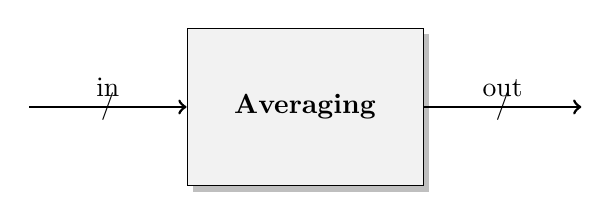
\begin{tikzpicture}
\node[block,rectangle,minimum height=2cm,minimum width=3cm] (bloc) {\textbf{Averaging}};

\path[connect,<-] ([yshift=0.0cm]bloc.west) -- node{/} node[above]{in} ++(-2cm,0);

\path[connect,->] ([yshift=0.0cm]bloc.east) -- node{/} node[above]{out} ++(2cm,0);
 ([xshift=0.5cm,yshift=-0.6cm]bloc.north);

\end{tikzpicture}
\end{figure}

\vspace{1.5cm}

\begin{figure}[!h]
\centering
\includegraphics[width=10cm]{averagingfilter.png}
\end{figure}

\section*{Properties}
\properties{
enable & bool & Enable the processing \\ 
}

\vspace{1.5cm}

\section*{Constants}

\constants{
LINE\_WIDTH\_MAX & Maximum line size of the image : 1280 pixels  \\ 
CLK\_PROC\_FREQ & Frequency clock of the process \\
IN\_SIZE & Size of the input flow : 1 byte \\
OUT\_SIZE & Size of the output flow : 1 byte  \\
WEIGHT\_SIZE & Size of the Kernel : 1 byte  \\
}

\vspace{1.5cm}

\section*{Equivalence}
\subsection*{Matlab}

\lstset{language=Matlab}
\begin{lstlisting}
I; % image matrix 3x3
K = [1 1 1 ; 1 1 1 ; 1 1 1]; % kernel 3x3
I_sobel = conv2(I,K); % convolved matrix image 

% SOBEL = edge(I, 'sobel'); 
	% Edge detection using 
	% Sobel operator

\end{lstlisting}

\vspace{1.5cm}

\section*{Mathematical formalism}


The idea of the averaging filtering is to replace each pixel value in an image with the average value of its neighbors to get an 3-by-3 matrix. This matrix is convoluted with the Kernel matrix $\kappa$, defined as follow : \\ 

\begin{equation}\label{eq1}
\kappa = \frac{1}{9} . \begin{pmatrix}
1 & 1 & 1 \\ 
1 & 1 & 1 \\ 
1 & 1 & 1
\end{pmatrix}
\end{equation}

\vspace{0.5cm}

Let's define the 3-by-3 matrix containing the neighbors pixels as follow :\\

\begin{equation}\label{eq2}
I = \begin{pmatrix}
i_{00} & i_{01} & i_{02} \\ 
i_{10} & i_{11} & i_{12} \\ 
i_{20} & i_{21} & i_{22}
\end{pmatrix}
\end{equation}

\vspace{0.5cm}

Let's convolute (\ref{eq1}) and (\ref{eq2}) :\\

\begin{equation}
\begin{matrix}
output ~ pixel = \kappa * I = \frac{1}{9} . \begin{pmatrix}
1 & 1 & 1 \\ 
1 & 1 & 1 \\ 
1 & 1 & 1
\end{pmatrix} * \begin{pmatrix}
i_{00} & i_{01} & i_{02} \\ 
i_{10} & i_{11} & i_{12} \\ 
i_{20} & i_{21} & i_{22}
\end{pmatrix}  \\ 
  \\
= \frac{1}{9}.(i_{00}+i_{01}+i_{02}+i_{10}+i_{11}+i_{12}+i_{20}+i_{21}+i_{22})
\end{matrix}
\end{equation}




\end{document}